\documentclass{report}
\usepackage[margin=1in, paperwidth=8.5in, paperheight=11in]{geometry}
%Math packages%
\usepackage{amsmath}
\usepackage{amsthm}
%Spacing%
\usepackage{setspace}
%Package to adjust indentation%
\usepackage{changepage}
\onehalfspacing
%Lecture number%
\newcommand{\lectureNum}{15}
%Variables - Date and Course%
\newcommand{\curDate}{March 2, 2017}
\newcommand{\course}{CS 240}
%Defining the example tag%
%\theoremstyle{definition}%
\newtheorem{ex}{Example}[section]
%Setting counter given the lecture number%
\setcounter{chapter}{\lectureNum{}}
%Package to insert code%
\usepackage{listings}
\usepackage{courier}
\usepackage{xcolor}
\lstset { 
    tabsize=2,
    breaklines=true,
    language=C++,
    backgroundcolor=\color{blue!8}, % set backgroundcolor
    basicstyle=\footnotesize\ttfamily,% basic font setting
}
%Package to draw trees%
\usepackage{tikz}


\begin{document}
%Note title%
\begin{center}
\begin{Large}
\textsc{\course{} | Lecture \lectureNum{}}
\end{Large}
\end{center} 
\noindent \textit{Bartosz Antczak} \hfill
\textit{Instructor: Eric Schost} \hfill
\textit{\curDate{}}
\rule{\textwidth}{0.4pt}

% Actual Notes%
\section{2-Dimensional Range Search}
Each item in a 2-D data structure has two \textit{aspects}: ($x_i,y_i$). This coordinate corresponds to a point in the Euclidean plane. There are various ways for implementing $d-$dimensional dictionaries:
\begin{itemize}
\item Reduce it to a one-dimensional dictionary
\item Use several dictionaries: one for each dimension
\item Use a \textit{partition tree} (quadtree, kd-tree)
\item Use multi-dimensional \textit{range trees}
\end{itemize}
\subsection{Quadtrees}
We have $n$ points $P = \{(x_0,y_0), (x_1,y_1), \cdots, (x_{n-1},y_{n-1})\}$. We build a quadtree on $P$ using these steps:
\begin{itemize}
\item Find a square $R$ that contains all the points of $P$. This corresponds to the root of the quadtree
\item Now \textbf{partition} $R$ into four equal subsquares (quadrants), each correspond to a child of $R$
\item Recursively repeat this process for any node that contains more than one point
\item The points that are on the split lines belong to the bottom left side. Also, any leaf not containing a point can be deleted
\end{itemize}
\begin{ex}
Building a sample quadtree
\end{ex}
\begin{figure}[ht]
\begin{center}
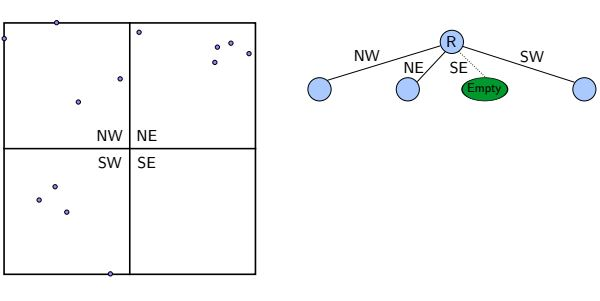
\includegraphics[scale=0.55]{quadtree.jpg}
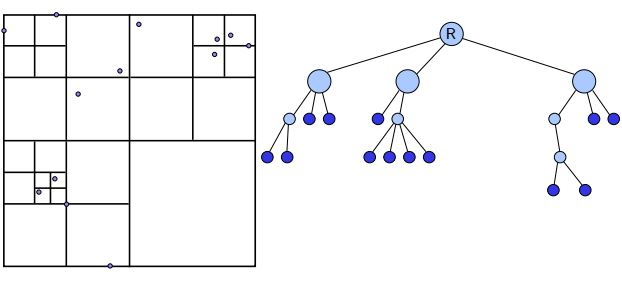
\includegraphics[scale=0.45]{quadtree2.jpg}
\end{center}
\caption{Building a quadtree. \textit{Courtesy of the CS 240 lecture slides.}}
\end{figure}
\newpage
\subsection{Quadtree Operations}
\subsubsection{Search}
It's analogous to BST search
\subsubsection{Insert}
\begin{itemize}
\item Search for the point
\item Split the leaf if there are two points
\end{itemize}
\subsubsection{Delete}
\begin{itemize}
\item Search for the point
\item Remove the point
\item If its parent has only one child left, delete that child and continue the process toward the root
\end{itemize}
\subsection{Quadtree Range Search}
The algorithm to find a particular range in a quadtree is
\begin{figure}[ht]
\begin{center}
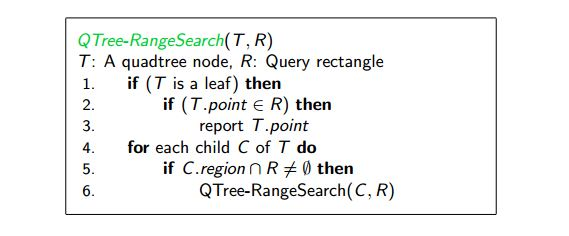
\includegraphics[scale=0.6]{algo1.jpg}
\end{center}
\caption{\textit{Courtesy of the CS 240 lecture slides.}}
\end{figure}
The complexity of range search is $\Theta(nh)$.
\subsection{The Height of a Quadtree}
We call $d_{max}$ the max distance between 2 points in $P$. The \textbf{height}  of a quadtree is $$h \in \Theta\left(\log_2 \displaystyle\left(\frac{d_{max}}{d_{min}}\right)\right)$$
\subsubsection{Proof of the Height of a Quadtree}
\textbf{Remarks:}
\begin{itemize}
\item Rescaling does not change the quadtree
\item Rescaling does not change the ratio $\frac{d_{max}}{d_{min}}$
\end{itemize}
From these remarks, we can assume that after rescaling, the bounding square has side length 1. We rescale to simplify the proof.
We call $d_{max}^\prime$ the \textbf{max} distance after rescaling, and we call $d_{min}^\prime$ the \textbf{min} distance after rescaling. From our previous remarks, observe that:
$$\frac{d_{max}^\prime}{d_{min}^\prime} = \frac{d_{max}}{d_{min}}$$
In any square $S$ of side length $c$, the max distance between 2 points, $P_1,P_2$, is $c\sqrt{2}$
\begin{center}
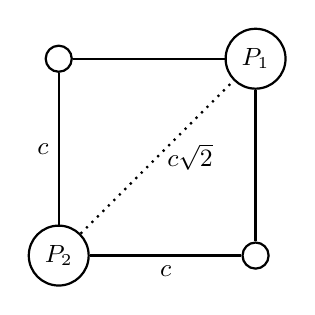
\begin{tikzpicture}[-,auto,node distance=2.5cm,
                    thick,main node/.style={circle,draw,font=\sffamily\small}]

  \node[main node] (1) {};
  \node[main node] (2) [right of=1] {$P_1$};
  \node[main node] (3) [below of=1] {$P_2$};
  \node[main node] (4) [right of=3] {};
  \path[every node/.style={font=\sffamily\small}]
    (1) edge (2)
    	edge node [left] {$c$} (3)
    (4) edge (2)
    	edge node [below] {$c$} (3)
    (3) edge [dotted] node [right] {$c\sqrt{2}$} (2);
\end{tikzpicture}
\end{center}
Note that $1 \leq d_{max}^\prime \leq \sqrt{2}$.\\After 1 level of subdivision, the squares have side length $\displaystyle\frac{1}{2}$. After 2 levels, it's $\displaystyle\frac{1}{2^2}$, and so on. In general, after $h$ levels, the square has side length $\displaystyle\frac{1}{2^h}$.
We stop once every square has only one point.
\\ Now, if $\displaystyle\frac{\sqrt{2}}{2^i} < d_{min}^\prime$, we must stop. If we have two points in this square, their distance is at most $\displaystyle\frac{\sqrt{2}}{2^i}$. This cannot happen, which is why we stop. So the height $h$ of the tree is at most the 1st integer $h$ such that
$$2^h \geq \frac{\sqrt{2}}{d_{min}^\prime}$$
So the height is in $O\left(\log\left(\displaystyle \frac{\sqrt{2}}{d_{min}^\prime}\right)\right)$. Observe that:
\begin{align*}
O\left(\log\left(\displaystyle \frac{\sqrt{2}}{d_{min}^\prime}\right)\right) &= O\left(\log\left(\displaystyle \frac{1}{d_{min}^\prime}\right)\right) \\
&= O\left(\log\left(\displaystyle \frac{d_{max}^\prime}{d_{min}^\prime}\right)\right) & (\text{Since} 1 \leq d_{max}^\prime \leq \sqrt{2}) \qed
\end{align*}
\subsection{KD-trees}
We have $n$ points $P = \{(x_0,y_0), (x_1,y_1), \cdots, (x_{n-1},y_{n-1})\}$. Unlike quadtrees, which splits a square into quadrants regardless of where points actually lie, a kd-tree splits the points into two (roughly) equal subsets. We build a kd-tree using these steps:
\begin{itemize}
\item Split $p$ into two equal subsets using a vertical line
\item Split each of the two subsets into two equal pieces using horizontal lines
\item Continue splitting, alternating vertical and horizontal lines, until every point is in a separate region
\item \textbf{Notes:}
\begin{itemize}
\item We initially sort the $n$ points according to their $x-$coordinate
\item The root of the tree is the point with median $x$ coordinate (its index is $\lfloor \frac{n}{2}\rfloor$ in the sorted list)
\item All other points with $x$ coordinate to the left of the point are smaller or equal in value; the points to the right are larger (exactly how a tree should be structured)
\end{itemize} 
\end{itemize}
These steps have a complexity of $\Theta(n \log n)$, and its height is $\Theta(\log n)$
\begin{ex}
Building a sample kd-tree on 10 points
\end{ex}
\begin{figure}[ht]
\begin{center}
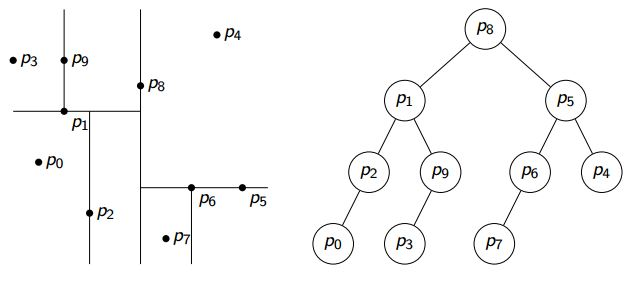
\includegraphics[scale=0.6]{kdtree.jpg}
\end{center}
\caption{\textit{Courtesy of the CS 240 lecture slides.}}
\end{figure}
%.....
Let $T(n)$ be the runtime for creating a kd-tree. Observe that:
$$T(n) = O(n \log n) + T^\prime(n)$$
It's broken down into sorting ($n \log n$) and the recursion ($T^\prime$).
$$T^\prime(n) = 2T^\prime\left(\frac{n}{2}\right) + O(n)$$
We see that $T^\prime(n) = O(n \log n)$. So the runtime becomes:
$$T(n) = O(n \log n) + O(n \log n) \in O(n \log n)$$
\subsection{KD Range Search}
The algorithm to find a particular range in the kd-tree is:
\begin{figure}[ht]
\begin{center}
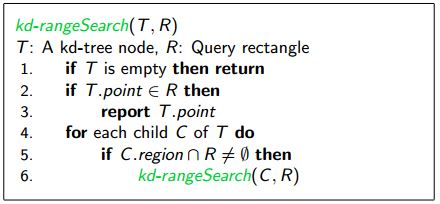
\includegraphics[scale=0.6]{range2.jpg}
\end{center}
\caption{\textit{Courtesy of the CS 240 lecture slides.}}
\end{figure}
\textit{More on this algorithm next lecture.}
%END%
\end{document}